\section{Shellsort}
O Shellsort foi desenvolvido por Donald L. Shell e apresentado em 1959 no artigo \textit{A High-Speed Sorting Procedure}. Trata-se de um método de ordenação não estável que se baseia na escolha de uma sequência de incrementos $h$ e, para cada valor $h_i$, do maior para o menor, transforma o vetor de entrada em um vetor $h_i$-ordenado.

\begin{definition}
No contexto do algoritmo Shellsort, uma sequência de incrementos é uma sequência de números inteiros positivos $h = \{h_1, h_2, ..., h_r\}$, tal que $h_1 = 1$ e $h_i < h_{i + 1}$.
\end{definition}

A análise de complexidade do Shellsort não é uma tarefa simples e depende da sequência de incrementos escolhida. Diversos pesquisadores propuseram diferentes sequências ao longo dos anos; algumas das mais conhecidas são mostradas na Tabela \ref{tab:shell-sort-increment-sequences}.

\begin{table}[H]
    \centering
    \Caption{\label{tab:shell-sort-increment-sequences}Sequências de incrementos}
    \begin{tabular}{| c | l | l | }
        \hline
        Referência & Sequência & Pior caso \\
        \hline
        % Donald L. Shell 
        \cite{shell1959high} & \( h_i = \lfloor n/2^i \rfloor \) & $\Theta(n^2)$ \\[6pt]
        
        % Thomas N. Hibbard 
        \cite{hibbard1963empirical} & \( h_i = 2^i - 1 \) & $\Theta(n^{3/2})$ \\[6pt]
        
        % Donald E. Knuth 
        \cite{knuth1973art} & \( h_i = (3^i - 1)/2 \) & $\Theta(n^{3/2})$ \\[6pt]

        % Robert Sedgewick 
        \cite{sedgewick1986new} & \( h_i = 4^i + 3 \times 2^{i-1} + 1 \) & \bigO{n^{4/3}} \\[6pt]
        
        % Naoyuki Tokuda 
        \cite{10.5555/645569.659879} & \( h_i = \left\lceil \frac{9(9/4)^i-4}{5} \right\rceil \) & - \\[6pt]
        
        % Marcin G. Ciura 
        \cite{ciura2001best} & $1, 4, 10, 23, 57, 132, 301, 701, 1750$ & - \\[6pt]
        \hline
    \end{tabular}
\end{table}

Neste trabalho é utilizada a sequência proposta por \cite{ciura2001best}. Tal sequência não possui uma análise precisa de complexidade de pior caso, mas demonstrou um bom desempenho experimentalmente, superando todas as outras. Os primeiros oito termos da sequência, escolhidos empiricamente pelo autor, são os mostrados na Tabela \ref{tab:shell-sort-increment-sequences}. Para expandir a sequência, uma abordagem comum é seguir a fórmula:  
\[
h_i = \lfloor 2,25 \times h_{i-1} \rfloor
\]

Desta forma, para a implementação do Shellsort mostrada em linguagem C abaixo, considere que o vetor \textit{CiuraSeq} foi criado de forma global e contém os primeiros $24$ termos da sequência descrita acima, em ordem decrescente.

\lstinputlisting[language=C]{codigos/sup/1_shellsort.txt}

\begin{figure}[H]
\Caption{\label{fig:shellsort}Estado de um vetor durante iterações do Shellsort.}
\centering
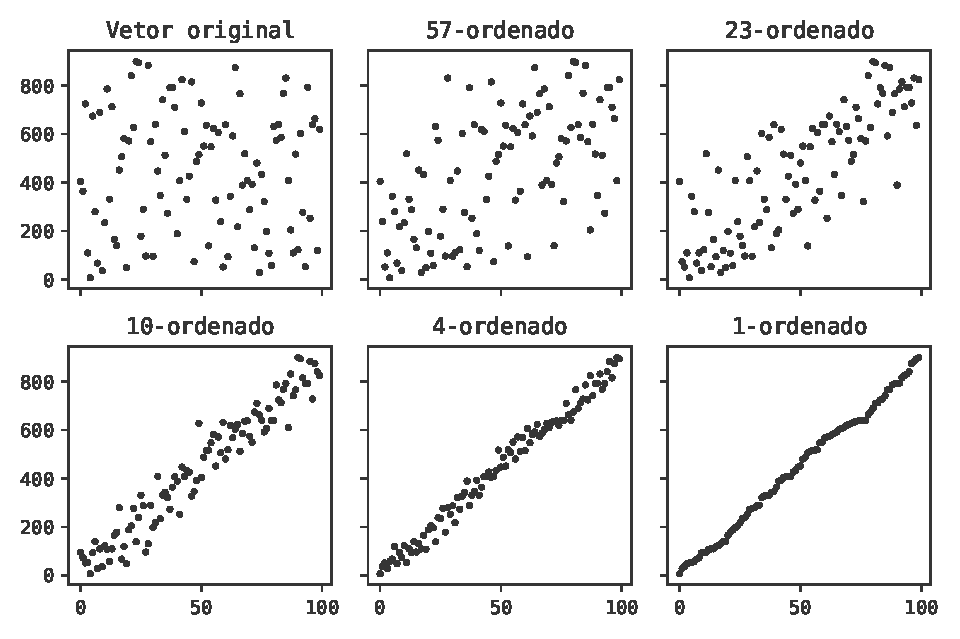
\includegraphics[scale=0.9]{figuras/pdf/shellsort.pdf}
\Fonte{Elaborado pelo autor}
\end{figure}
